\chapter{開発環境}
\label{chap:concept}

\section{iOSアプリケーション}
本研究では, Mac OS Xに搭載されている開発ツールスイートであるXcodeを用いてiOSアプリケーションを開発する.

\subsection{Objective-C}
Objective-Cとは, C言語をベースとして開発されたプログラミング言語である.

\begin{quotation}
“NEXTSTEP\footnote{NeXTコンピュータに搭載されたオブジェクト指向マルチタスクオペレーションシステム.}とMac OS X\footnote{Machintoshコンピュータに搭載されているオペレーティング・システム.}に標準付属されており, 現在は主にMac OS XとiOS上で動作するアプリケーションを開発する際に利用されている.
Objective-CはGCCによってコンパイル可能であるため, 基本的にはUNIX, Linix系OSや, GCCコンパイラを使用できる環境であればプログラムを動作させることが可能である.“

“C言語にSmalltalkをマクロ的拡張として施した言語であり, C言語により近い拡張を施されたC++と異なり, C言語とオブジェクト指向が混在した言語であると述べるほうが適切である.”

“if/for/whileなどの制御文や, int/char/floatなどのスカラー型, 関数記法, 宣言や代入といった基本的な文法はC言語に準拠しているが, オブジェクト指向はSmalltalkの概念を借用したものであり, その大きな特徴である「メッセージパッシングによるメソッド呼び出しを利用した, 記述力に優れたオブジェクトシステム」を継承している.”
\end{quotation}
\begin{flushright}
(出典:\url{https://ja.wikipedia.org/wiki/Objective-C})
\end{flushright}

\begin{description}
\item (A) Objective-Cの特徴

Objective-Cによるオブジェクト指向開発環境[2]は, 以下の3要素から成り立つ.

\begin{description}
\item a) オブジェクト

\begin{quotation}
“オブジェクト指向言語を利用したプログラムは, オブジェクトと呼ばれる要素を中心に構成される.
オブジェクトとは, データと, そのデータを利用したりデータに作用する特定の関数による操作を関連付けたものをいう.
これらの操作はオブジェクトのメソッドと呼ばれる.
メソッドが作用するデータをインスタンス変数という.”

“よって, オブジェクトはインスタンス変数とメソッドを, 自己完結型のプログラミング単位にまとめたものと言い換えることができる.”

“Objective-Cでは, オブジェクトのインスタンス変数はオブジェクト内に存在し, 一般には, オブジェクトのメソッドによってのみ作用される.”

“他のメソッドがインスタンス変数に格納されているデータを得るには, アクセスしたいインスタンス変数を内包しているオブジェクトが, データを提供するメソッドを実装していなければならないが, インスタンス変数の有効範囲を指定することで, サブクラスや他のオブジェクトからインスタンス変数に直接アクセスすることも可能である.”
\end{quotation}
\begin{flushright}
(出典:\url{https://developer.apple.com/jp/documentation/ObjC.pdf})
\end{flushright}

\item b) 開発ツールスイート

\begin{quotation}
“Objective-Cで開発を行うための開発ツールとして代表的なものに, Xcodeが挙げられる.”

“Xcodeは, Apple Inc.が開発, 配布している, Mac/iPhone/iPad/Apple Watch向けアプリケーション開発用のデベロッパツールセットである.”

“ユーザインターフェースのデザイン, コーディング, テスト, デバッグ, Apple Storeへの提出を行えることによる, スムーズなアプリケーション開発を実現している.”

“また, Xcodeには, Xcode IDE(統合開発環境:Integrated Development Environment), SwiftおよびObjective-Cのプログラミング言語向けコンパイラ, Instruments分析ツール, iOS Simukator, 最新のiOS/OS X向けSDKなどの機能も用意されている.”
\end{quotation}
\begin{flushright}
(出典:\url{https://developer.apple.com/jp/documentation/ObjC.pdf})
\end{flushright}

\item c) ランタイム環境

\begin{quotation}
“Objective-Cでは, 可能な限り多くの決定が実行時に行われる.
オブジェクトの作成やどのメソッドを呼び出すかの決定などの動作は動的に実行されるため, Objective-Cでは, コンパイラだけでなく, コンパイルしたコードを実行するランタイムシステムも必要となる.

“ランタイムシステムは, Objective-Cにとって, 一種のオペレーティングシステムとして動作し, 言語を機能させる.”
\end{quotation}
\begin{flushright}
(出典:\url{https://developer.apple.com/jp/documentation/ObjC.pdf})
\end{flushright}

\end{description}

\item (B) Objective-C 2.0

Apple Inc.はMac OS X v10.5 Leopardにおいて, 言語仕様を変更したObjective-C 2.0を発表した.
Objective-C 2.0では, ガベージコレクションとプロパティの導入, foreach文の採用, 実装オプションのプロトコル定義の増加, 非公開プライベートメソッドが実装可能, ランタイム構造の変更などが行われた.
\end{description}

\subsection{OpenCV}
OpenCV(Open Source Computer Vision Library)とは, Intel Corporationが開発, 公開しているオープンソースのコンピュータビジョン用ライブラリである.

\begin{quotation}
“画像処理, 画像解析, 機械学習の機能を持つC/C++, Java, Python, MATLAB用ライブラリで, プラットフォームとしてUnix/Linux系OS, Windows, Android, iOSなどをサポートしている.
BSDライセンスで配布されているため, 学術目的のみでなく, 商用目的でも利用することが可能である.”
\end{quotation}
\begin{flushright}
(出典:\url{https://ja.wikipedia.org/wiki/OpenCV})
\end{flushright}

1999年に開発プロジェクトが開始され, 2000年のアルファ版公開を皮切りに, 2001年から2005年にかけて, 5つのベータ版が公開されている.
正式版のリリース後, 2016年1月現在まで開発, 公開されている(表2.1).

\begin{table}[tb]
\begin{center}
\begin{tabular}{|l|l|l|} \hline
バージョン & リリース年月 & 公式サポート言語 \\ \hline \hline
1.0 & 2006年10月 & C言語 \\ \hline
2.0 & 2009年10月 & C言語, C++ \\ \hline
2.1 & 2010年4月 & C言語, C++ \\ \hline
2.2 & 2010年12月 & C言語, C++, Python \\ \hline
2.3 & 2011年7月 & C言語, C++, Python \\ \hline
2.4 & 2012年5月 & C言語, C++, Python \\ \hline
2.4.1 & 2012年6月 & C言語, C++, Python \\ \hline
2.4.2 & 2012年7月 & C言語, C++, Python \\ \hline
2.4.3 & 2012年11月 & C言語, C++, Python \\ \hline
2.4.4 & 2013年3月 & C言語, C++, Python, Java \\ \hline
2.4.5 & 2013年4月 & C言語, C++, Python, Java \\ \hline
2.4.6 & 2013年7月 & C言語, C++, Python, Java \\ \hline
2.4.7 & 2013年11月 & C言語, C++, Python, Java \\ \hline
2.4.8 & 2013年12月 & C言語, C++, Python, Java \\ \hline
2.4.9 & 2014年4月 & C言語, C++, Python, Java \\ \hline
2.4.10 & 2014年10月 & C言語, C++, Python, Java \\ \hline
2.4.11 & 2015年2月 & C言語, C++, Python, Java \\ \hline
3.0 & 2015年6月 & C++, Python, Java(3.0以降, C言語はメンテナンス対象外) \\ \hline
3.1 & 2015年12月 & C++, Python, Java \\ \hline
\end{tabular}
\caption{OpenCVのバージョンとリリース年月, 公式サポート言語の一覧}
\end{center}
\end{table}

最新バージョンであるOpenCV 3.x系列では, C言語関数形式のインターフェイスがメンテナンス対象外とされ, C++ APIを利用することが推奨されている.

\begin{description}
\item (A) OpenCVの機能

OpenCVに実装されている機能としては, フィルター処理, 変形処理, 構造解析と形状ディスクリプタ, 物体検出, モーション解析と物体追跡, 領域分割, カメラキャリブレーション, 特徴点検出, 機械学習がある[4].

\begin{description}
\item a) フィルター処理

OpenCVにおけるフィルタリングは, 二次元配列であるMat型で定義された二次元画像に対して処理を実行する.
画像の平滑化や収縮/膨張などの処理を行うことで, 画像のぼかしやノイズキャンセリングを施す.

\item b) 変形処理

二次元画像の幾何学変換を行い, 変形画像をマッピングする.
この処理を施す際は画像の内容そのものは変更されず, ピクセルの座標移動のみを行う..

\item c) 構造解析と形状ディスクリプタ

二次元画像内に描かれている, あるいは含まれている特定の形状を検出する.
画像内の特定の形状のみを認識したい場合等で利用する.

\item d) 物体検出

予め設定しているテンプレートと二次元画像とを比較し, テンプレートとマッチングする物体を検出する.
顔認識や指紋認識など, 生体認証等で利用する.

\item e) モーション解析と物体追跡

動画内で動いている物体の動きを認識する, あるいは動体を追跡する.
モーション検知や動体検知等で利用する.

\item f) 領域分割

二次元画像を形状や色などの特徴を用いて, 複数の領域に分割する.
特定の領域のみで画像処理を施す場合や, 特定の領域のみを抜き出す場合等で利用する.

\item g) カメラキャリブレーション

カメラ固有の内部パラメータと, ワールド座標系における位置や姿勢を意味する外部パラメータを求める.
カメラで撮影した二次元画像の歪みを補正する場合等で利用する.

\item h) 特徴点検出

二次元画像における特徴点を検出する.
特徴点を検出してパターンマッチングを行う場合等で利用する.

\item i) 機械学習

OpenCVでは, ニューラルネットワークを用いた機械学習を実装することが可能である.
二次元画像を教師データとして入力し, 形状や物体の認識率を向上させる場合等で利用する.
\end{description}

\end{description}

\subsection{Tesseract-OCR}
Tesseract-OCRとは, ヒューレット・パッカード研究所とヒューレット・パッカード社が開発し, 現在はGoogleが開発, 配布している, 光学文字認識用のオープンソースライブラリである.

ライブラリの大半はC言語で書かれており, 一部はC++で書かれている.
そのため, C言語コンパイラがインストールされているならば, 様々な環境で動作させる事ができる.

Tesseract-OCRは2016年1月現在, 64の言語に対応している(表2.2).

\begin{table}[tb]
\begin{center}
\begin{tabular}{|p{3.5cm}|p{3.5cm}|p{3.5cm}|p{3.5cm}|} \hline
英語 & ウクライナ語 & トルコ語 & タイ語 \\ \hline
タガログ語 & テルグ語 & タミル語 & スウェーデン語 \\ \hline
スワヒリ語 & セルビア語 & アルバニア語 & スペイン古語 \\ \hline
スペイン語 & スロベニア語 & スロバキア語 & ローマ語 \\ \hline
ポルトガル語 & ポーランド語 & ノルウェー語 & オランダ語 \\ \hline
マレー語 & マルタ語 & マケドニア語 & マラヤーラム語 \\ \hline
リトアニア語 & ラトビア語 & 韓国語 & カナダ語 \\ \hline
イタリア古語 & イタリア語 & アイスランド語 & インドネシア語 \\ \hline
チェロキー語 & ハンガリー語 & クロアチア語 & ヒンディー語 \\ \hline
ヘブライ語 & ガルシア語 & 中世フランス語 & フランス語 \\ \hline
フランク語 & フィン語 & バスク語 & エストニア語 \\ \hline
エスペラント語 & 中世英語 & グリーク語 & ドイツ語 \\ \hline
デンマーク語 & チェコ語 & カタロニア語 & ブルガリア語 \\ \hline
ブルガリア語 & ベンガル語 & ベラルーシ語 & アゼルバイジャン語 \\ \hline
アラビア語 & アフリカ語 & 日本語 & 中国語(簡体字) \\ \hline
中国語(繁体字) & ロシア語 & ベトナム語 & 数学記号 \\ \hline
\end{tabular}
\caption{Tesseract-OCRにて認識可能な言語一覧}
\end{center}
\end{table}

Tesseract-OCRはニューロンネットワークによる機械学習を実装しており, 上記の言語のデータを教師データとして与えることにより, 文字の認識率を向上させることが可能である.

\section{Webアプリケーション}
本研究では, Rubyで開発されたWebアプリケーションフレームワークで高いシェアを誇るRuby on Railsを用いてWebアプリケーションを開発する.

Webアプリケーションの開発環境は, 琉球大学工学部情報工学科が管理, 提供しているVPSサーバに構築した.

\section{VPSサーバの環境}
\subsection{CentOS}
CentOSとは, The CentOS Projectがオープンソースライセンスで開発, 配布しているLinixディストリビューションである.

\begin{quotation}
“CentOSという名称は「コミュニティベースで開発された, 有償版に匹敵するオペレーティングシステム(Community ENTerprise Operating System)」が由来となっている.”

“2004年5月のリリースから, RHELの最新版が公開される度に, その後を追うようにしてメジャーアップデートを重ね, 2016年1月現在まで開発, 配布されている.”

“Red Hat Enterprise Linux(RHEL)\footnote{Red Hat社が開発, 販売している業務向けLinuxディストリビューション.}の完全互換を目指して開発され, Red Hat社がオープンソースにて公開しているRHELのソースコードを基に, Red Hat社の商標や商用パッケージを除去し, リビルドしたものがCentOSである.
このことから, CentOSは一般に「RHELクローン」\footnote{RHELを基としたLinuxディストリビューション全般を含んだ呼称であるため, White Box Enterprise LinuxやScientific LinuxもRHELクローンに含まれる.}と呼称されることもある.”
\end{quotation}
\begin{flushright}
(出典:\url{https://ja.wikipedia.org/wiki/CentOS})
\end{flushright}

Linuxをベースとしたオペレーティングシステムであること, GNUライセンスによる配布による低コストでの導入の容易さから, 主に中小規模のプロジェクトにて採用されることが多い.

\subsection{Ruby on Rails}
Ruby on Railsとは, Rails Core Teamが開発, 提供しているオープンソースのWebアプリケーションフレームワークである.

オブジェクト指向スクリプト言語であるRubyにて記述されており, オブジェクト指向を強く意識したフレームワークとなっている.

2004年10月に正式版がリリースされてから, 2016年1月現在まで開発, 公開されている.

\begin{comment}
\begin{table}[tb]
\begin{center}
\begin{tabular}{|l|l|} \hline
バージョン & リリース年月 \\ \hline \hline
0.8.0 & 2004年10月 \\ \hline
0.9.0 & 2004年12月 \\ \hline
0.10.0 & 2005年2月 \\ \hline
0.11.0 & 2005年3月 \\ \hline
0.12.0 & 2005年4月 \\ \hline
0.13.0 & 2005年7月 \\ \hline
0.14.1 & 2005年10月 \\ \hline
1.0.0 & 2005年12月 \\ \hline
1.1.0 & 2006年3月 \\ \hline
1.2.0 & 2007年1月 \\ \hline
2.0.0 & 2007年12月 \\ \hline
2.1.0 & 2008年5月 \\ \hline
2.2.2 & 2009年11月 \\ \hline
2.3.2 & 2009年5月 \\ \hline
3.0.0 & 2010年8月 \\ \hline
3.1.0 & 2011年8月 \\ \hline
3.2.0 & 2012年1月 \\ \hline
4.0.0 & 2013年6月 \\ \hline
4.1.0 & 2014年4月 \\ \hline
4.2.0 & 2014年12月 \\ \hline
4.2.5 & 2015年11月 \\ \hline
\end{tabular}
\caption{Ruby on Railsのメジャーバージョンとリリース年月の一覧}
\end{center}
\end{table}
\end{comment}

\begin{description}
\item (A)Webアプリケーションフレームワーク

\begin{quotation}
“Webアプリケーションフレームワークとは, 動的なウェブサイト, Webアプリケーション, Webサービスの開発をサポートするために設計されたアプリケーションフレームワークである.”

“アプリケーションフレームワークとは, 特定のオペレーティングシステムのためのアプリケーションの標準構造を実装するのに使われるクラスやライブラリの集合である.”
\end{quotation}
\begin{flushright}
(出典:\url{https://ja.wikipedia.org/wiki/Ruby_on_Rails})
\end{flushright}

つまり, 端的にWebアプリケーションフレームワークを言い換えると, Webアプリケーションを開発する際に必要なクラスやライブラリを提供する, Webアプリケーションの土台となるものとなる.

HTMLやPHP等の, Webページ/アプリケーションを開発するための言語を扱うことに長けた専門家が, それらの言語を用いて一から開発したアプリケーションと同等のものが, Webアプリケーションフレームワークを用いることで, 初心者でも開発することが可能となる[5].

\item (B) Ruby on Railsの特徴

Ruby on Railsの特徴は, その開発理念である“同じことを繰り返さない(DRY:Don't Repeat Yourself)”と'“設定より規約(CoC:Convention over Configuration)”の順守による, 実アプリケーションの開発が他のフレームワークよりも少ないコードで簡単に行える点である.

“同じことを繰り返さない”とは, 「定義などの作業は一度のみ行う」, 「重複するコードを記述しない」という意味である.

“設定より規約”とは, 「慎重に設定された規約に従うことで, 設定を不要にする, あるいは軽減する」という意味である.

これらの基本理念により, Ruby on Railsでは, コンソール上でコマンドを入力することで, 命名規則に従った複数の関連付けられたファイルが生成されるため, ファイル構成の把握が非常に簡易である.

このRuby on Railsのコンセプトに影響を受けたフレームワークとして, PHPのCakePHPやSymfony, PerlのCatalyst, JavaのGrailsといったものが挙げられる.

\item (C) Ruby on RailsにおけるMVCアーキテクチャ

Ruby on RailsはMVC(Model View Controller)アーキテクチャを採用している.

\begin{quotation}
“MVCアーキテクチャとは, アプリケーションの構造をModel/View/Controllerの3つの要素に分割し, アプリケーションの内部データを利用者が直接参照することがないようにしたものである(図2.1).”
\end{quotation}
\begin{flushright}
(出展:\url{https://ja.wikipedia.org/wiki/Model_View_Controller})
\end{flushright}

\begin{figure}
\begin{center}
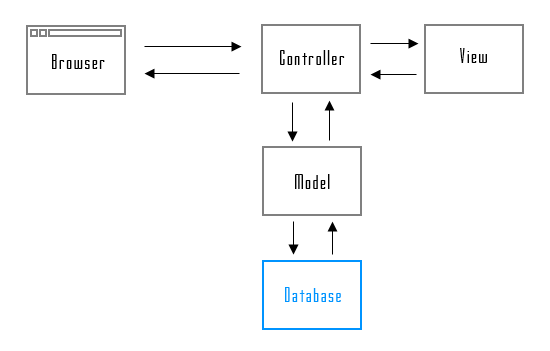
\includegraphics[width=13cm]{fig/mvc.png}
\caption{MVCアーキテクチャの簡略図}
\end{center}
\begin{flushright}
(出展:\url{http://www.rubylife.jp/rails/ini/index7.html})
\end{flushright}
\end{figure}

\begin{itemize}
\item Model

\begin{quotation}
“アプリケーションが扱う領域のデータと手続きを表現した要素.
データの変更をビューに通知するのもModelの役割である.”
\end{quotation}
\begin{flushright}
(出展:\url{https://ja.wikipedia.org/wiki/Model_View_Controller})
\end{flushright}

\begin{quotation}
“Ruby on RailsにおけるModelは, 使用しているデータベースのテーブルごとにModelが用意されている.
利用者からのリクエストで呼びだされたアクションは, Modelを介してデータベースとのやり取りを行い, データの取得や新しいデータの格納を行う(図2.2).”
\end{quotation}
\begin{flushright}
(出典:\url{http://www.rubylife.jp/rails/ini/index7.html})
\end{flushright}

\begin{figure}
\begin{center}
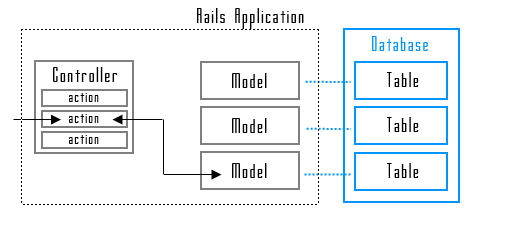
\includegraphics[width=13cm]{fig/model.png}
\caption{Modelの動作簡略図}
\begin{flushright}
(\url{http://www.rubylife.jp/rails/ini/index7.html})
\end{flushright}
\end{center}
\end{figure}

\item View

\begin{quotation}
“Modelのデータを取り出し, ユーザが見るのに適した形となるHTML文書を作成する要素.
すなわち, データをブラウザへ出力するための雛形を作成するのが役割である.”
\end{quotation}
\begin{flushright}
(出典:\url{https://ja.wikipedia.org/wiki/Model_View_Controller})
\end{flushright}

\begin{quotation}
“Ruby on RailsにおけるViewは, アプリケーション内に複数用意されている.
Viewの1つ1つが与えられたデータから生成されたHTML文書となっている.
アクションに対応するViewが1つ用意されており, アクションが実行されると, 紐付けされたViewが呼び出されて利用者へ返すWebページを作成する(図2.3).”
\end{quotation}
\begin{flushright}
(出典:\url{http://www.rubylife.jp/rails/ini/index7.html})
\end{flushright}

\begin{figure}
\begin{center}
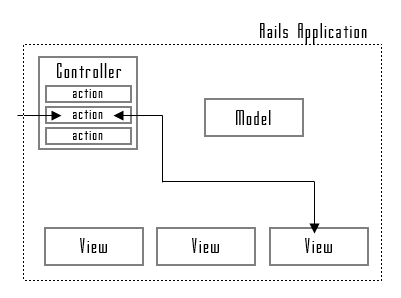
\includegraphics[width=13cm]{fig/view.png}
\caption{Viewの動作簡略図}
\end{center}
\begin{flushright}
(出典:\url{http://www.rubylife.jp/rails/ini/index7.html})
\end{flushright}
\end{figure}

\item Controller

\begin{quotation}
“ユーザからの入力をModelへのメッセージに変換し, 伝える要素である.
すなわち, UIからの入力を担当する.”
\end{quotation}
\begin{flushright}
(出典:\url{https://ja.wikipedia.org/wiki/Model_View_Controller})
\end{flushright}

\begin{quotation}
“Ruby on RailsにおけるControllerは, アプリケーション内に複数用意されている.
また, 各Controllerの中には複数のアクションが定義されており, URLとして届いた利用者のリクエストを分析し, どのControllerに含まれるどのアクションを実行すべきか判断するための「ルーティング」が行われる(図2.4).”
\end{quotation}
\begin{flushright}
(出典:\url{http://www.rubylife.jp/rails/ini/index7.html})
\end{flushright}

\begin{figure}
\begin{center}
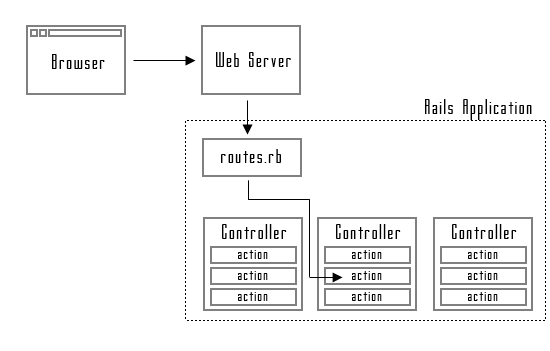
\includegraphics[width=13cm]{fig/route.png}
\caption{ルーティング}
\end{center}
\begin{flushright}
(\url{http://www.rubylife.jp/rails/ini/index7.html})
\end{flushright}
\end{figure}

\begin{quotation}
“ルーティングによって次に行われるべきアクションが決定した際, そのアクションに紐付けされたModelがデータベースとのやり取りを, Viewがユーザへ返すHTML文書を作成する.
返ってきたHTML文書をControllerがリクエストした利用者に見える形でブラウザに返す(図2.5).”
\end{quotation}
\begin{flushright}
(出典:\url{http://www.rubylife.jp/rails/ini/index7.html})
\end{flushright}

\begin{figure}
\begin{center}
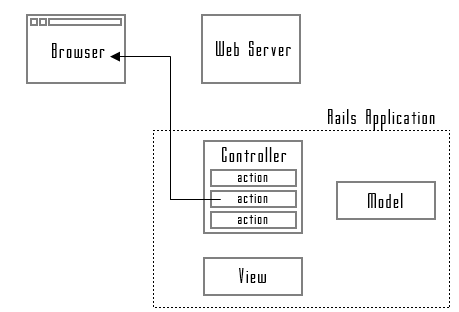
\includegraphics[width=13cm]{fig/controller.png}
\caption{Controllerの動作簡略図}
\end{center}
\begin{flushright}
(\url{http://www.rubylife.jp/rails/ini/index7.html})
\end{flushright}
\end{figure}

\end{itemize}

\end{description}

\subsection{PostgreSQL}
PostgreSQLとは, PostgreSQL Global Development Groupがオープンソースで開発, 配布している, オブジェクト関係データベース管理システム(ORDBMS:Objective Relational DataBase Management System)である.

1995年5月に正式版がリリースされてから, 2016年1月現在まで開発, 公開されている(表2.4).

\begin{comment}
\begin{table}[tb]
\begin{center}
\begin{tabular}{|l|l|} \hline
バージョン & リリース年月 \\ \hline \hline
0.01 & 1995年5月 \\ \hline
1.0 & 1995年9月 \\ \hline
6.0 & 1997年1月 \\ \hline
6.1 & 1997年6月 \\ \hline
6.2 & 1997年10月 \\ \hline
6.3 & 1998年3月 \\ \hline
6.4 & 1998年10月 \\ \hline
6.5 & 1999年6月 \\ \hline
7.0 & 2000年5月 \\ \hline
7.1 & 2001年4月 \\ \hline
7.2 & 2002年2月 \\ \hline
7.2 & 2002年11月 \\ \hline
7.4 & 2003年11月 \\ \hline
8.0 & 2005年1月 \\ \hline
8.1 & 2005年11月 \\ \hline
8.2 & 2006年12月 \\ \hline
8.3 & 2008年2月 \\ \hline
8.4 & 2009年7月 \\ \hline
9.0 & 2010年9月 \\ \hline
9.1 & 2011年9月 \\ \hline
9.2 & 2012年9月 \\ \hline
9.3 & 2013年9月 \\ \hline
9.4 & 2014年12月 \\ \hline
9.5 & 2016年1月 \\ \hline
\end{tabular}
\caption{PostgreSQLのメジャーバージョンとリリース年月の一覧}
\end{center}
\end{table}
\end{comment}

PostgreSQLは, オープンソースなリレーショナルデータベース管理システム(RDBMS)であるIngresから発展したプロジェクトである.

\begin{quotation}
“PostgreSQLという名は, 「Post-Ingres」, つまり「Ingresの後継であること」と, 「SQLデータベース操作構文を用いてデータベース操作が可能であること」が, その名の由来となっている.
Ingresの課題であった, 「ユーザが新たな定義域を既存の単純な定義域から定義できない」という実装の限界に対処することを目的として開発された.”

“データベースの操作にはSQLデータベース操作構文を利用しているが, PL/pgSQL, PL/PSM, スクリプト言語(PL/Perl, PL/php, PL/Python, PL/Ruby, PL/Tcl, PL/Lua), コンパイラ言語(C言語, PL/Java), 統計処理言語(PL/R)の関数を実行することも可能である.”
\end{quotation}
\begin{flushright}
(出典:\url{https://ja.wikipedia.org/wiki/PostgreSQL})
\end{flushright}

\begin{description}
\item (A) リレーショナルデータベース(Relational DataBase)

\begin{quotation}
“リレーショナルデータベースとは, 一見のデータを複数の属性(カラム)の値(フィールド)の組(レコード)として表現し, 組を列挙することでデータを格納していく方式のデータベースのことである.
属性を列, 組を業とする表(テーブル)の形で表されることが多い.
複数のテーブルに含まれる同じカラムを関連付けることができ, 複雑なデータや大規模なデータを柔軟に取り扱うことができる.”
\end{quotation}
\begin{flushright}
(出典:\url{http://e-words.jp/w/RDBMS.html})
\end{flushright}

データベースの構造では最も普及しており, 単にデータベースといった場合はリレーショナルデータベースであることが多い.

\item (B) Relational DataBase Management System

Relational DataBase Management System(RDBMS)とは, リレーショナルデータベースを管理するための専用ソフトウェアである.

\begin{quotation}
“ストレージ内に専用の管理領域を確保し, テーブルの作成や消去, 構造の修正, データの追加, 検索, 抽出, 修正, 削除等を行う.
データベース管理者や利用者が直接操作を行う他に, 外部のソフトウェアから接続を受け付け, ソフトウェアのプログラムから操作を行うことも可能である.
RDBMSへの照会や操作の指示には, SQLと呼ばれるデータベース操作言語が標準として広く利用されている.”

“RDBMSは, 不正なデータの記録を拒否するなどしてデータベースの整合性を保つ, 権限のない利用者による不正な読み出しや改ざん等からデータを保護する等の仕組みを持つ.
また, 関連する複数の処理を一体化して矛盾なく実行するトランザクション処理を行ったり, 障害に備えてデータベースのバックアップを行い, 破損時には過去のある時点の状態へと復旧したりといった機能を備えたものもある.”
\end{quotation}
\begin{flushright}
(出典:\url{http://e-words.jp/w/RDBMS.html})
\end{flushright}

\end{description}

\subsection{Heroku}
Herokuとは, 2007年に創業された同名の企業が開発と運営を行っている, PaaS(Platform as a Service)である.

Herokuは自社の目的として, “技術者をビジネスの本質的な価値提供(アプリケーション開発)に集中させること”, “開発者の生産性を最大化すること”を掲げており, PaaSの提供だけでなく, 高頻度の機能追加やアドオンの提供を行っている.

PaaSとは, アプリケーションを実行するためのプラットフォームである.

“アプリケーションを実行するためのプラットフォーム”は, 「ハードウェア」, 「ネットワーク」, 「仮想化環境」, 「オペレーティングシステム」, 「データベース」, 「アプリケーションフレームワーク」で構成されている.

Webアプリケーションを自らの手で一から全て開発する場合,
\begin{enumerate}
\item サーバPCやルータ等のハードウェアを購入

\item それらをインターネットに接続し, かつプライベート空間を分離するためのファイアウォールを含むネットワークを構築

\item サーバの仮想化環境を整備

\item LinuxやWindowsサーバ等のオペレーティングシステムをインストール

\item OracleやMySQL, PostgreSQL等のデータベースをセットアップ

\item JavaやRuby, PHP等のアプリケーション実行環境をセットアップ
\end{enumerate}

という手順を踏んで, アプリケーションを公開するための環境を整えなければならない.

PaaSは, これらのプラットフォームの構築にかかる様々な作業を代行してくれるサービスである.
PaaSを利用することで, 最初に行わなければならない環境構築への労力を軽減し, また, プラットフォームの保守運用にかかる費用を削減することが可能となる.

Webアプリケーション開発の補助を行うサービスとして, 「IaaS(Infrastructure as a Service)」, 「SaaS(Software as a Service)」があり, そして全てを自ら管理する「オンプレミス」がある(図2.1).

\begin{figure}
\begin{center}
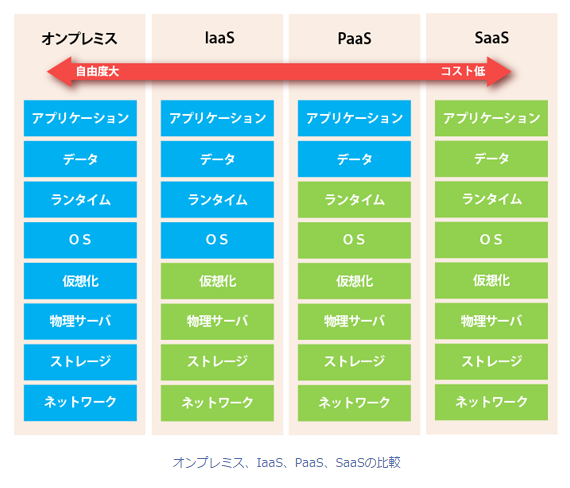
\includegraphics[width=16cm]{fig/paas.png}
\caption{オンプレミス, IaaS, PaaS, SaaSの比較}
\end{center}
\begin{flushright}
(\url{http://codezine.jp/article/detail/8051})
\end{flushright}
\end{figure}

\begin{itemize}
\item オンプレミス

プラットフォームの全てを自身で管理する.

「ハードウェア」, 「ネットワーク」, 「仮想化環境」, 「オペレーティングシステム」, 「データベース」, 「アプリケーションフレームワーク」を自身で選択できるため, 開発の自由度が高い.

しかし, 環境構築からアプリケーション公開までの労力は必然的に重たくなる.

\item IaaS

プラットフォームのうち, 「ハードウェア」, 「ネットワーク」, 「仮想化環境」までをサービス事業者が管理する.

「オペレーションシステム」, 「データベース」, 「アプリケーションフレームワーク」は自ら選択できるため, サービス利用者の慣れ親しんだ環境でのアプリケーション開発を行うことができる.

\item PaaS

プラットフォームの「ハードウェア」, 「ネットワーク」, 「仮想化環境」, 「オペレーティングシステム」, 「データベース」までをサービス事業者が管理する.

「アプリケーションフレームワーク」にて開発したアプリケーションをサービス会社のサーバにアップロードすることで, サービス事業者がランタイム(アプリケーションの実行)まで行う.

サービス利用者はアプリケーションの開発, 運用のみに注力すればよいが, 開発環境の自由度はIaaSよりも低い.

\item SaaS

プラットフォームの全てをサービス事業者が管理する.

管理コストは最も低いが, 開発環境の自由度も低い.

サービス事業者が提供するソフトウェアをインストールして利用する形態を採用しているため, サービス事業者によって開発可能なサービスが異なる可能性がある.
\end{itemize}

本研究では, Webアプリケーションをインターネット上で公開する際に利用するサービスとして, PaaSを提供しているHerokuを採用する.

その理由として,  「仮想環境の構築までは予め用意されている環境を使用し, Webアプリケーションは自ら選択したフレームワークで開発する」ためである.
また, 高頻度の機能追加や多種多様なアドオンの提供を実施しており, 開発環境を整えやすいのもHerokuを採用した理由の一つである.
